%%%%%%%%%%%%%%%%%%%%%%%%%%%%%%%%%%%%%%%%%%%%%%%%%%%%%%%%%%%%%%%%%%%%%
% by Mahamdi Amine
%%%%%%%%%%%%%%%%%%%%%%%%%%%%%%%%%%%%%%%%%%%%%%%%%%%%%%%%%%%%%%%%%%%%%%
\documentclass[12pt]{report}
\usepackage[T1]{fontenc}
\usepackage{lmodern}
\usepackage[a4paper]{geometry}
\usepackage[myheadings]{fullpage}
\usepackage{fancyhdr}
\usepackage{lastpage}
\usepackage{hyperref}
\usepackage{graphicx, wrapfig, subcaption, setspace, booktabs}
\usepackage[T1]{fontenc}
\usepackage[font=small, labelfont=bf]{caption}
\usepackage[protrusion=true, expansion=true]{microtype}
\usepackage[english]{babel}
\usepackage{sectsty}
\usepackage{hyperref}
\usepackage{listings}
\hypersetup{
    colorlinks,
    citecolor=black,
    filecolor=black,
    linkcolor=black,
    urlcolor=black
}
\usepackage{url, lipsum}
\usepackage[utf8]{inputenc}
\usepackage{indentfirst}
\newcommand{\HRule}[1]{\rule{\linewidth}{#1}}
\onehalfspacing
\setcounter{tocdepth}{5}
\setcounter{secnumdepth}{5}
\pagestyle{fancy}
\fancyhf{}
\setlength\headheight{15pt}
\fancyhead[L]{fm\char`_mahamdi@esi.dz    }
\fancyhead[R]{fm\char`_leghettas@esi.dz}
\fancyfoot[R]{Page \thepage\ sur \pageref{LastPage}}
\usepackage{placeins}
\begin{document}
%\renewcommand{\contentsname}{Table des Matières}
%\renewcommand{\listfigurename}{Table des Figures}
\author{MAHAMDI Mohammed  LEGHETTAS Mohamed-Hicham  }       
\date{} 
\title{  \textsc{ Chess with Neural Network .}
		\\ [2.0cm]
		\HRule{0.5pt} \\
		\LARGE \textbf{\uppercase{Project Report
				. }}
		\HRule{2pt} \\ [0.5cm]
		\normalsize \today \vspace*{5\baselineskip}}
\maketitle
\tableofcontents
\newpage
\listoffigures 
\newpage
\sectionfont{\scshape}
\newpage
\chapter{Introduction}

\chapter{Theoratical study}
	\section{Biological	Neurons}
		\begin{figure}[h!]
			\centering
			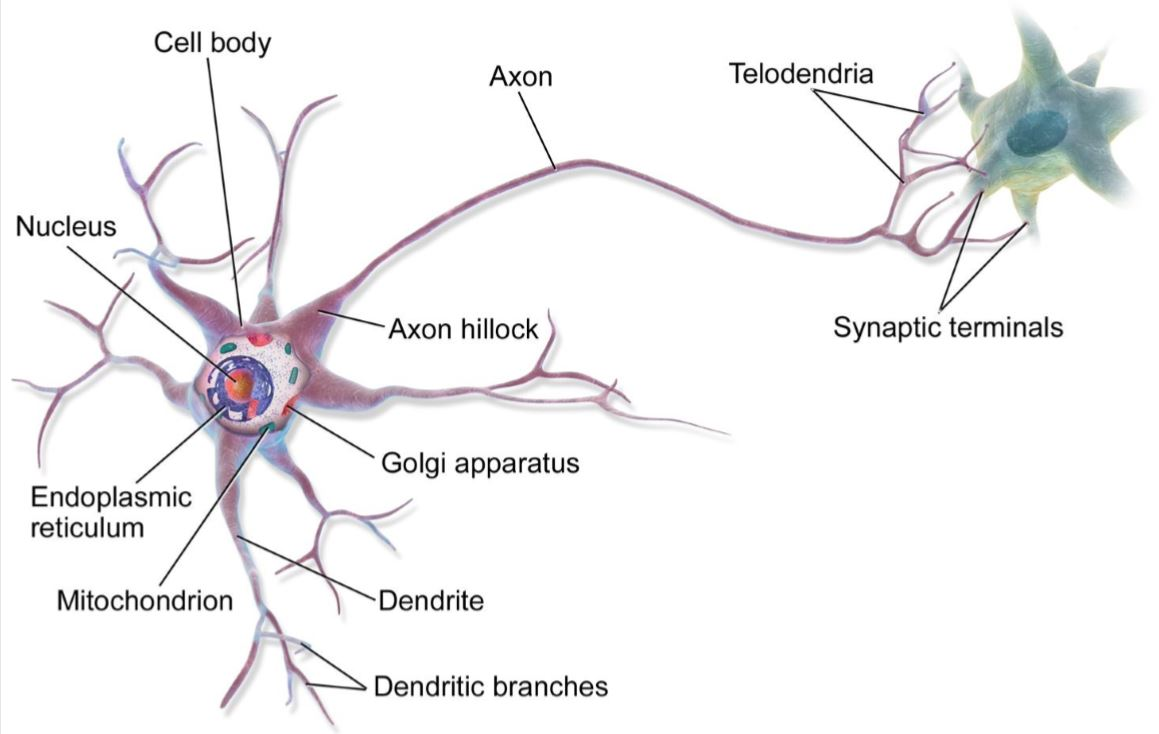
\includegraphics[scale=1, width=15cm]{./images/BiologicalNeurons.jpg}
			\caption{title1.}	
		\end{figure}
		\FloatBarrier
		
		\section{Logical Computations with Neuron}
		\begin{figure}[h!]
			\centering
			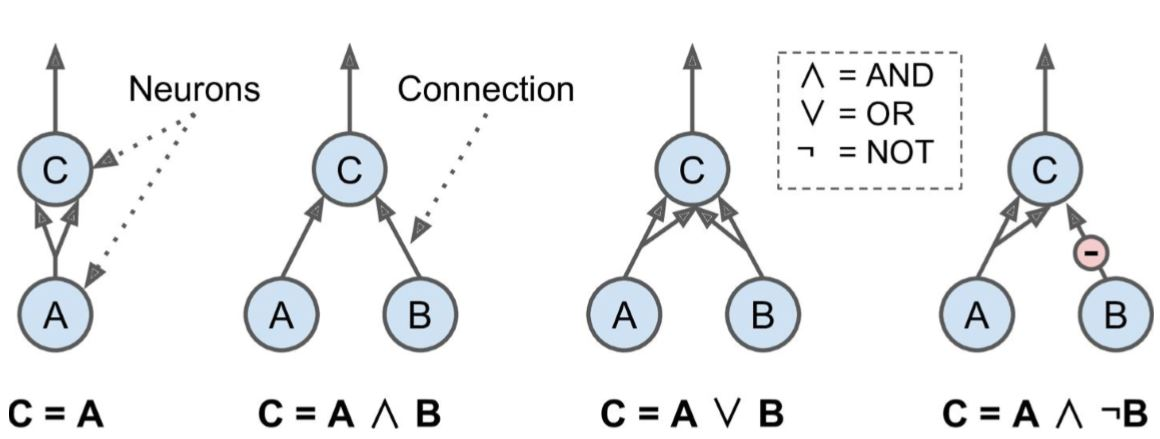
\includegraphics[scale=1, width=15cm]{./images/LogicalComputationswithNeuron.jpg}
			\caption{title2.}	
		\end{figure}
		\FloatBarrier
		
\chapter{Technical realization}

	\section{The choice of programming language}
		We can realize this work with almost all the well knowing programming languages such a :C,C++,C#,Java,Python ...
		\newline
		There are a number of reasons why the Python programming language is popular with professionals who work on machine learning systems:
		\begin{enumerate}
			\item	\textbf{Readability and less complexity :}\\
			You can easily understand it and make someone understand very fast.
			\item	\textbf{Packages everywhere !}\\
			Numpy,scikit,librosa,pandas,matplotlib,tensorflow, pytorch,Django ...
			\item	\textbf{many features that are attractive for scientific computing :}\\
			Python has a simple and consistent syntax which makes programming more accessible to people who are not software engineers.
		\end{enumerate}	
	\section{Choosing framework for building Neural Networks}
		\begin{itemize}
			\item Tensorflow and PyTorch are open-source.
			\item the computational graphs.
			\item Tensorflow has a more steep learning curve than PyTorch.
			\item Tensorflow has a much bigger community behind it than PyTorch.
			\item Pytorch is so easy to debug.
	\end{itemize}
	\section{Web View}
	\section{Chess Library}
	\section{The Code with the other Tools}
\chapter{conclusion}

\end{document}
